%Version 3.1 December 2024
\documentclass[pdflatex, sn-nature]{sn-jnl}

%%%% Standard Packages
\usepackage{graphicx}%
\usepackage{multirow}%
\usepackage{amsmath,amssymb,amsfonts}%
\usepackage{amsthm}%
\usepackage{mathrsfs}%
\usepackage[title]{appendix}%
\usepackage{xcolor}%
\usepackage{textcomp}%
\usepackage{manyfoot}%
\usepackage{booktabs}%
\usepackage{algorithm}%
\usepackage{algorithmicx}%
\usepackage{algpseudocode}%
\usepackage{listings}%
\usepackage{siunitx}
%%%%

\theoremstyle{thmstyleone}%
\newtheorem{theorem}{Theorem}%
\newtheorem{proposition}[theorem]{Proposition}% 

\theoremstyle{thmstyletwo}%
\newtheorem{example}{Example}%
\newtheorem{remark}{Remark}%

\theoremstyle{thmstylethree}%
\newtheorem{definition}{Definition}%

\graphicspath{{../Image/MS/}}

\raggedbottom

\begin{document}

\title[]{Spatiotemporal Interference of Cutaneous Shear Waves Dictates Tactile Perception in Ultrasonic Haptics}

\author[1]{\fnm{Linhan} \sur{Fan}}\email{linhanfan@seu.edu.cn}

\author[1]{\fnm{Zhutao} \sur{Wang}}\email{xxxx@seu.edu.cn}

\author*[1]{\fnm{Yafeng} \sur{Niu}}\email{nyf@seu.edu.cn}

\affil*[1]{\orgdiv{School of Mechanical Engineering}, \orgname{Southeast University}, \orgaddress{\city{Nanjing}, \country{China}}}

\abstract{}

\maketitle

\section{Introduction}\label{sec:intro}

\section{Results}\label{sec:results}

\begin{figure}
    \centering
    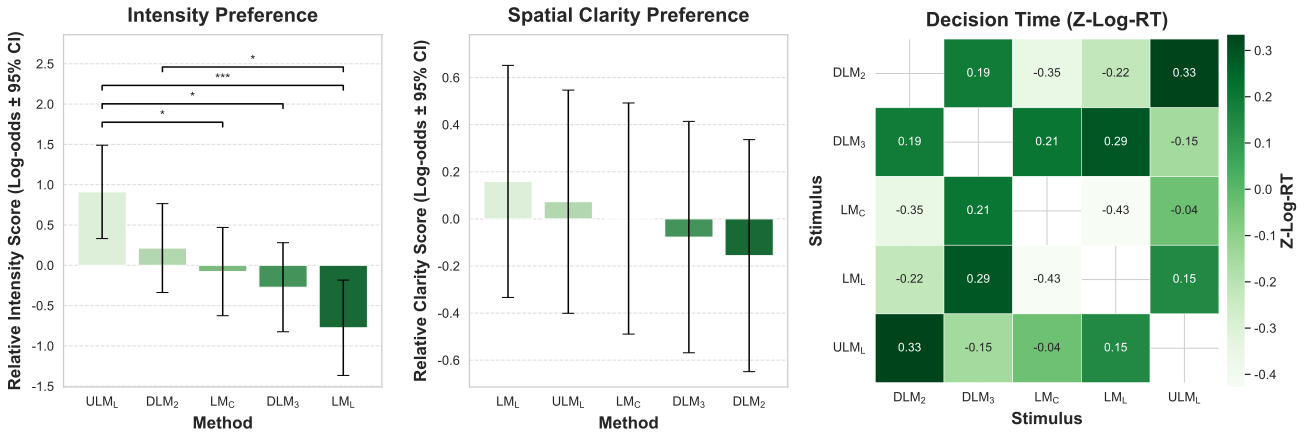
\includegraphics[width= \textwidth]{Graph/Experiment 1 Combined.pdf}
    \caption{Combined plot of Relative intensity, clarity, and Reaction Time results.}
    \label{fig:combined_plot}
\end{figure}

\section{Discussion}\label{sec:discussion}

\section{Methods}\label{sec:methods}

\backmatter

\section*{Acknowledgments}
This work was supported jointly by National Natural Science Foundation of China (72571059), the SEU Innovation Capability Enhancement Plan for Doctoral Students (CXJH\_SEU 26066).

\bibliography{SWIM}% common bib file

\end{document}
